\section{Page d'accueil des administrateurs}
\label{sec::home_admin}

\begin{figure}[H]
	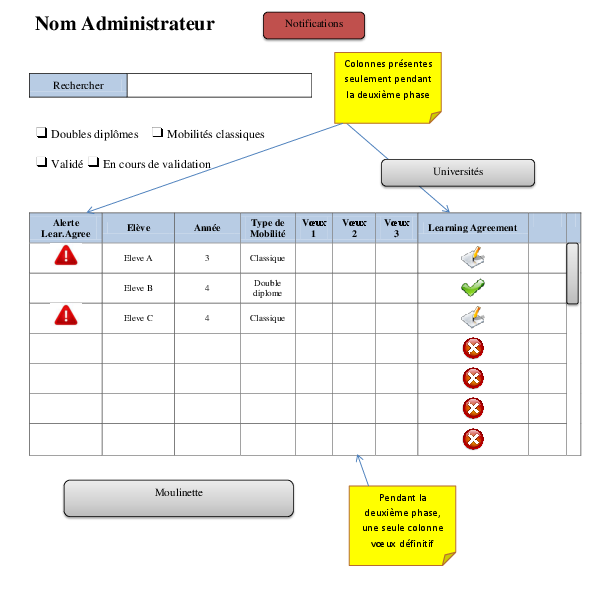
\includegraphics[scale=0.7]{Admin/HomeAd.png}
	\caption{Page d'accueil des administrateurs}
\end{figure}

C'est sur cette pas qu'un Administrateur arrive après sa connection au CAS. Cette page va servir à gérer durant la phase de vœux, les vœux des élèves mais aussi les documents déposés par les élèves lors de la seconde phase.

Le principal élément de cette page est un tableau regroupant:
\begin{itemize}
 	\item le nom des élèves
 	\item l'année de l'élève
 	\item si l'élève souhaite une mobilité classique ou double diplôme
 	\item une case précisant si les vœux de l'élèves sont définitif ou non (en phase 1)
 	\item une case précisant l'état de l'élève (learning agreement en attente, en cours de validation, validé) (en phase 2)
 	\item la liste des voeux de l'élève (en phase 1)
 	\item le voeux de l'élève (en phase 2)
 	\item une case d'alerte prévenant du dépôt d'un learning agreement à valider
 \end{itemize}
 
Dans le tableau, le nom des élèves est un lien vers leur page d'accueil sur laquelle l'administrateur peut aller en mode admin. Cela lui permet de modifier les vœux d'un élève par le biais de son compte.

Les voeux de l'élèves sont aussi des lien ramenant sur la page des universités en mode administrateur.Cela lui permet notamment d'ajouter de nouvelles université ou de mettre des commentaire professeur sur une université existante

Au dessus du tableau, l'administrateur pourra utiliser une barre de recherche par mot clé ainsi que des filtres (learning agreement en attente de walidation, learning agreement validé, double diplôme,mobilité classique,année d'étude de l'élève).\\

Aussi présent en haut de la page une case de notification des learning agreement récemment déposés. Le fait de cliquer sur cette case nous emmène au tableau sur lequel un filtre est ajouter pour ne voir que les élèves concernés.\\

On trouvera aussi un lien permettant à l'administrateur d'accéder à la liste des université mais en mode administrateur.\\

Enfin l'administrateur dispose d'un lien lui permettant d'accéder à la moulinette permettant à la fin de la phase de vœux de faire la répartition des destinations pour les élèves.